\documentclass[journal, a4paper]{IEEEtran}


\usepackage{graphicx}  
\usepackage{url}        
\usepackage{amsmath}

\begin{document}
	\title{Implementation of Random Forests}
	\author{Alejandro Su\'arez Hern\'andez}
	\markboth{Supervised and Experiential Learning}{}
	\maketitle

% Write abstract here
\begin{abstract}
	This report presents our implementation of Random Forests for
	classification and presents
	some exploratory results. Namely, we are interested in the performance
	of our classifier under different settings, varying the number of
	features considered randomly at each decision stump and the size of the
	ensemble. Another interesting aspect of Random Forests that we will
	review in this document is that they perform implicit feature
	selection. We can take advantage of this to rank the input attributes
	according to their relevance predicting the output class.
\end{abstract}

% Each section begins with a \section{title} command
\section{Introduction}
	% \PARstart{}{} creates a tall first letter for this first paragraph
	\PARstart{R}{andom} forests is an ensemble method for both regression
	and classification. It essentially consists in learning several decision
	trees from the data, introducing some source of randomness
	in the learning process so they are not
	equal. When classifying a new instance, the forest aggregates the
	predictions of all the trees into a single answer. In the classification
	case, the aggregation method is typically the mode (i.e. the most
	frequently predicted class). In regression, the average of all the guesses
	is a common choice. In this document, we focus on the classification
	problem.
	
	These are the most frequent techniques to introduce stochasticity in the
	learning process:
	\begin{itemize}
		\item \textbf{Bootstrap aggregating:} also known as bagging. It is
		a general method that consists
		in training each learner (in our case, each tree) with a
		random sample of the original train data.
		\item \textbf{Feature bagging:} when learning, select the best
		splitting feature from a random sample of features. Each
		selected feature is splitted optimally according to some
		information criterion (entropy, Gini impurity, error...). The number
		of random features to consider is a parameter of the algorithm.
		This technique is explored in this document.
		\item \textbf{Random splits:} take randomization even one step
		further making the local splits random as well. That is, the
		information criterion is used exclusivelly to select the best
		randomly splitted feature. This technique has been adopted by
		the ExtraTrees (Extremely Randomized Trees) algorithm.
	\end{itemize}
	
	This document revolves around a custom implementation of Random Forests.
	It incorporates feature bagging and accepts several parameters in order
	to tweak its performance for each data set. More specifically:
	\begin{itemize}
		\item \textbf{Number of selected features ($F$):} the number of candidate
		features chosen randomly at each node for evaluation. $F$ is
		clipped if the number of available features is smaller.
		\item \textbf{Number of learners ($M$):} the number of trees in the
		ensemble.
		\item \textbf{Minimum number of instances to split ($N$):} the learner will
		continue splitting the current node if the number of instances that
		have arrived to it is at least $N$.
		\item \textbf{Split quality criterion:} the implementation
		accepts three criterions: (1) information
		gain (or entropy minimization); (2) Gini impurity coefficient; (3) 
		classification error or $ 1 - p_{max} $ where $ p_max $ is the probability
		of the most frequent class in the split.
	\end{itemize}
	
	Our implementation offers other features like the possibility of storing
	the learnt ensembles in a JSON file, and visualizing them via Graphviz.
	We refer the reader to the \texttt{README.md} file in this repository
	in order to know more about the technical details of our application
	\footnote{Github: \url{https://github.com/sprkrd/randomforest}}.
	
	In the next section we explore the prediction power of our classifier
	with different parametrizations. In addition, we analyze its ability
	to rank features based on their frequence of apparition as criterion
	in the decision stumps.

\section{Experiments}

\begin{table}[tbp]
\centering
\caption{Data sets used for testing our RF implementation}
\resizebox{\columnwidth}{!}{\begin{tabular}{|r|r|r|r|r|r|}
\hline
\textbf{Data set} & \textbf{Records} & \textbf{Nom. Attr.} & \textbf{Num. Attr} & \textbf{Classes} & \textbf{Missing(\%)} \\ \hline
Audiology & 226 & 69 & 0 & 24 & 2 \\ \hline
Credit & 690 & 9 & 6 & 2 & 0.6 \\ \hline
Hepatitits & 155 & 13 & 6 & 2 & 5.7 \\ \hline
Votes & 435 & 16 & 0 & 2 & 5.6 \\ \hline
Iris & 150 & 0 & 4 & 3 & 0 \\ \hline
Chess & 3196 & 36 & 0 & 2 & 0 \\ \hline
Lenses & 24 & 4 & 0 & 3 & 0 \\ \hline
Soybean & 47 & 35 & 0 & 4 & 0 \\ \hline
Splices & 3190 & 60 & 0 & 3 & 0 \\ \hline
Zoo & 101 & 16 & 1 & 7 & 0 \\ \hline
\end{tabular}}
\label{tab:datasets}
\end{table}

The tested data sets are shown in Table~\ref{tab:datasets}. We aim mostly at
studying the accuracy of the ensemble under different selections of $M$ (number
of trees) and $F$ (number of random features). For the sake of simplicity, the
rest of parameters will be fixed: $ N = 4 $; and the quality metric is the
Giny impurity. We invite the reader to experiment further with our application.

\subsection{Accuracy}

We have tested our ensemble model for $ M \in \{50, 100\} $ and for
$ F \in \{1, 3, \lfloor\log_2(N_{attr}+1)\rfloor, \left[\sqrt{N_{attr}}\right]\} $ (discarding
repeated values of $ F $).

The results are as follows:
\begin{itemize}
	\item \textbf{Audiology:} shown in Table~\ref{tab:acc-audiology}. There is a
	slight improvement for increasing $ M $ and $ F $.
	\item \textbf{Credit:} shown in Table~\ref{tab:acc-crx}. The accuracy does not
	seem to be affected.
	\item \textbf{Hepatitis:} shown in Table~\ref{tab:acc-hepatitis}. Surprisingly,
	the accuracy seems to be higher for the smallest value of $ F $.
	\item \textbf{Votes:} shown in Table~\ref{tab:acc-votes}. The best accuracy
	has been obtained with $ F = 4 $ and 100 learners.
	\item \textbf{Chess:} shown in Table~\ref{tab:acc-chess}. The difference between
	the best and the worst configuration is almost a 3\% with a very low
	deviation.
	\item \textbf{Lenses:} shown in Table~\ref{tab:acc-lenses}. Perhaps not a very
	relevant data set because of the low number of examples. The deviation is too
	high to draw conclusions.
	\item \textbf{Soybean:} shown in Table~\ref{tab:acc-soybean}. Perfect
	classification with all the configurations.
	\item \textbf{Splice:} shown in Table~\ref{tab:acc-splice}. One of the data
	sets in which the parameters choice have the most notable effect, jumping
	from a worst case accuracy of 87.81\% ($ M = 50 $ and $ F = 1 $) to
	96.39\% ($ M = 100 $ and $ F = 8 $). The deviation is also greatly
	reduced, suggesting that this is indeed a very stable configuration.
	\item \textbf{Zoo:} shown in Table~\ref{tab:acc-zoo}. The parameters do not
	have a very noticeable effect.
\end{itemize}

\begin{table}[htbp]
\caption{Accuracy results for Audiology data set}
\begin{center}
\begin{tabular}{|r|r|r|r|r|}
\hline
\textbf{M\textbackslash{}F} & \textbf{1} & \textbf{3} & \textbf{7} & \textbf{8} \\ \hline
\textbf{50} & 73.78 $ \pm $ 6.19 & 74.67 $ \pm $ 7.65 & 74.22 $ \pm $ 7.52 & 74.67 $ \pm $ 9.06 \\ \hline
\textbf{100} & 72.44 $ \pm $ 7.77 & 75.11 $ \pm $ 6.50 & 74.67 $ \pm $ 8.15 & 76.00 $ \pm $ 8.93 \\ \hline
\end{tabular}
\end{center}
\label{tab:acc-audiology}
\end{table}

\begin{table}[htbp]
\caption{Accuracy results for Credit Approval data set}
\begin{center}
\begin{tabular}{|r|r|r|r|}
\hline
\textbf{M\textbackslash{}F} & \textbf{1} & \textbf{3} & \textbf{4} \\ \hline
\textbf{50} & 86.52 $ \pm $ 2.36 & 85.65 $ \pm $ 1.86 & 86.38 $ \pm $ 1.68 \\ \hline
\textbf{100} & 86.67 $ \pm $ 2.27 & 86.96 $ \pm $ 1.02 & 86.23 $ \pm $ 2.00 \\ \hline
\end{tabular}
\end{center}
\label{tab:acc-crx}
\end{table}

\begin{table}[htbp]
\caption{Accuracy results for Hepatitis data set}
\begin{center}
\begin{tabular}{|r|r|r|r|r|}
\hline
\textbf{M\textbackslash{}F} & \multicolumn{1}{r|}{\textbf{1}} & \multicolumn{1}{r|}{\textbf{3}} & \multicolumn{1}{r|}{\textbf{4}} & \multicolumn{1}{r|}{\textbf{5}} \\ \hline
\textbf{50} & 82.58 $ \pm $ 3.29 & 81.29 $ \pm $ 3.76 & 82.58 $ \pm $ 1.58 & 82.58 $ \pm $ 4.83 \\ \hline
\textbf{100} & 85.16 $ \pm $ 2.58 & 84.52 $ \pm $ 1.29 & 81.94 $ \pm $ 4.38 & 80.65 $ \pm $ 5.40 \\ \hline
\end{tabular}
\end{center}
\label{tab:acc-hepatitis}
\end{table}

\begin{table}[htbp]
\caption{Accuracy results for Iris data set}
\begin{center}
\begin{tabular}{|r|r|r|r|}
\hline
\textbf{M\textbackslash{}F} & \textbf{1} & \textbf{2} & \textbf{3} \\ \hline
\textbf{50} & 93.33 $ \pm $ 4.71 & 93.33 $ \pm $ 4.71 & 94.67 $ \pm $ 2.67 \\ \hline
\textbf{100} & 94.00 $ \pm $ 4.90 & 94.00 $ \pm $ 4.90 & 94.67 $ \pm $ 2.67 \\ \hline
\end{tabular}
\end{center}
\label{tab:acc-iris}
\end{table}

\begin{table}[htbp]
\caption{Accuracy results for Votes data set}
\begin{center}
\begin{tabular}{|r|r|r|r|r|}
\hline
\textbf{M\textbackslash{}F} & \textbf{1} & \textbf{3} & \textbf{4} & \textbf{5} \\ \hline
\textbf{50} & 94.71 $ \pm $ 2.25 & 96.78 $ \pm $ 1.69 & 96.55 $ \pm $ 1.63 & 96.09 $ \pm $ 1.17 \\ \hline
\textbf{100} & 95.17 $ \pm $ 1.52 & 96.78 $ \pm $ 1.52 & 97.01 $ \pm $ 1.56 & 96.78 $ \pm $ 1.52 \\ \hline
\end{tabular}
\end{center}
\label{tab:acc-votes}
\end{table}

\begin{table}[htbp]
\caption{Accuracy results for Chess data set}
\begin{center}
\begin{tabular}{|r|r|r|r|}
\hline
\textbf{M\textbackslash{}F} & \textbf{1} & \textbf{3} & \textbf{6} \\ \hline
\textbf{50} & 96.87 $ \pm $ 0.75 & 99.03 $ \pm $ 0.35 & 99.56 $ \pm $ 0.15 \\ \hline
\textbf{100} & 97.18 $ \pm $ 0.57 & 99.19 $ \pm $ 0.44 & 99.53 $ \pm $ 0.17 \\ \hline
\end{tabular}
\end{center}
\label{tab:acc-chess}
\end{table}

\begin{table}[htbp]
\caption{Accuracy results for Lenses data set}
\begin{center}
\begin{tabular}{|r|r|r|r|}
\hline
\textbf{M\textbackslash{}F} & \textbf{1} & \textbf{2} & \textbf{3} \\ \hline
\textbf{50} & 75.00 $ \pm $ 15.81 & 85.00 $ \pm $ 12.25 & 85.00 $ \pm $ 12.25 \\ \hline
\textbf{100} & 70.00 $ \pm $ 18.71 & 85.00 $ \pm $ 12.25 & 85.00 $ \pm $ 12.25 \\ \hline
\end{tabular}
\end{center}
\label{tab:acc-lenses}
\end{table}

\begin{table}[htbp]
\caption{Accuracy results for Soybean data set}
\begin{center}
\begin{tabular}{|r|r|r|r|}
\hline
\textbf{M\textbackslash{}F} & \textbf{1} & \textbf{3} & \textbf{6} \\ \hline
\textbf{50} & 100.00 $ \pm $ 0.00 & 100.00 $ \pm $ 0.00 & 100.00 $ \pm $ 0.00 \\ \hline
\textbf{100} & 100.00 $ \pm $ 0.00 & 100.00 $ \pm $ 0.00 & 100.00 $ \pm $ 0.00 \\ \hline
\end{tabular}
\end{center}
\label{tab:acc-soybean}
\end{table}

\begin{table}[htbp]
\caption{Accuracy results for Splice data set}
\begin{center}
\begin{tabular}{|r|r|r|r|r|}
\hline
\textbf{M\textbackslash{}F} & \textbf{1} & \textbf{3} & \textbf{6} & \textbf{8} \\ \hline
\textbf{50} & 87.81 $ \pm $ 2.20 & 95.02 $ \pm $ 0.89 & 96.14 $ \pm $ 0.80 & 96.39 $ \pm $ 0.52 \\ \hline
\textbf{100} & 88.62 $ \pm $ 3.01 & 96.05 $ \pm $ 0.52 & 96.71 $ \pm $ 0.38 & 96.39 $ \pm $ 0.60 \\ \hline
\end{tabular}
\end{center}
\label{tab:acc-splice}
\end{table}

\begin{table}[htbp]
\caption{Accuracy results for Zoo data set}
\begin{center}
\begin{tabular}{|r|r|r|r|r|}
\hline
\textbf{M\textbackslash{}F} & \textbf{1} & \textbf{3} & \textbf{4} & \textbf{5} \\ \hline
\textbf{50} & 95.00 $ \pm $ 4.47 & 93.00 $ \pm $ 4.00 & 94.00 $ \pm $ 3.74 & 95.00 $ \pm $ 4.47 \\ \hline
\textbf{100} & 95.00 $ \pm $ 4.47 & 95.00 $ \pm $ 3.16 & 96.00 $ \pm $ 4.90 & 94.00 $ \pm $ 3.74 \\ \hline
\end{tabular}
\end{center}
\label{tab:acc-zoo}
\end{table}

\subsection{Feature ranking}

As said before, Random Forests are useful to sort the features of a data set according
to their relevance, as long as $ F > 1 $. Otherwise, at each node the chosen feature is
completely random. This is evidenced by the following example.

The ranking and scores for the Iris data set with $ M = 50 $ and $ F = 1 $ is:
\begin{enumerate}
\item sepal-length (0.27821)
\item sepal-width (0.266537)
\item petal-length (0.2393)
\item petal-width (0.215953)
\end{enumerate}

We can see that the scores do not actually differ too much. However, let us see what happens
maintaining the same value of $ M $, but with $ F = 3 $:

\begin{enumerate}
\item petal-length (0.445693)
\item petal-width (0.348315)
\item sepal-length (0.198502)
\item sepal-width (0.00749064)
\end{enumerate}

We can see that now petal-length and petal-width have gained much more relevance than the other
two features. In fact, this has much sense, since the petal-length alone can be used to discriminate
away one of the three classes. Not only this, but it plays a crucial role for discriminating
the remaining two. Fig.~\ref{fig:iris-tree} shows one of the learnt trees.

\begin{figure*}[htbp]
\centering
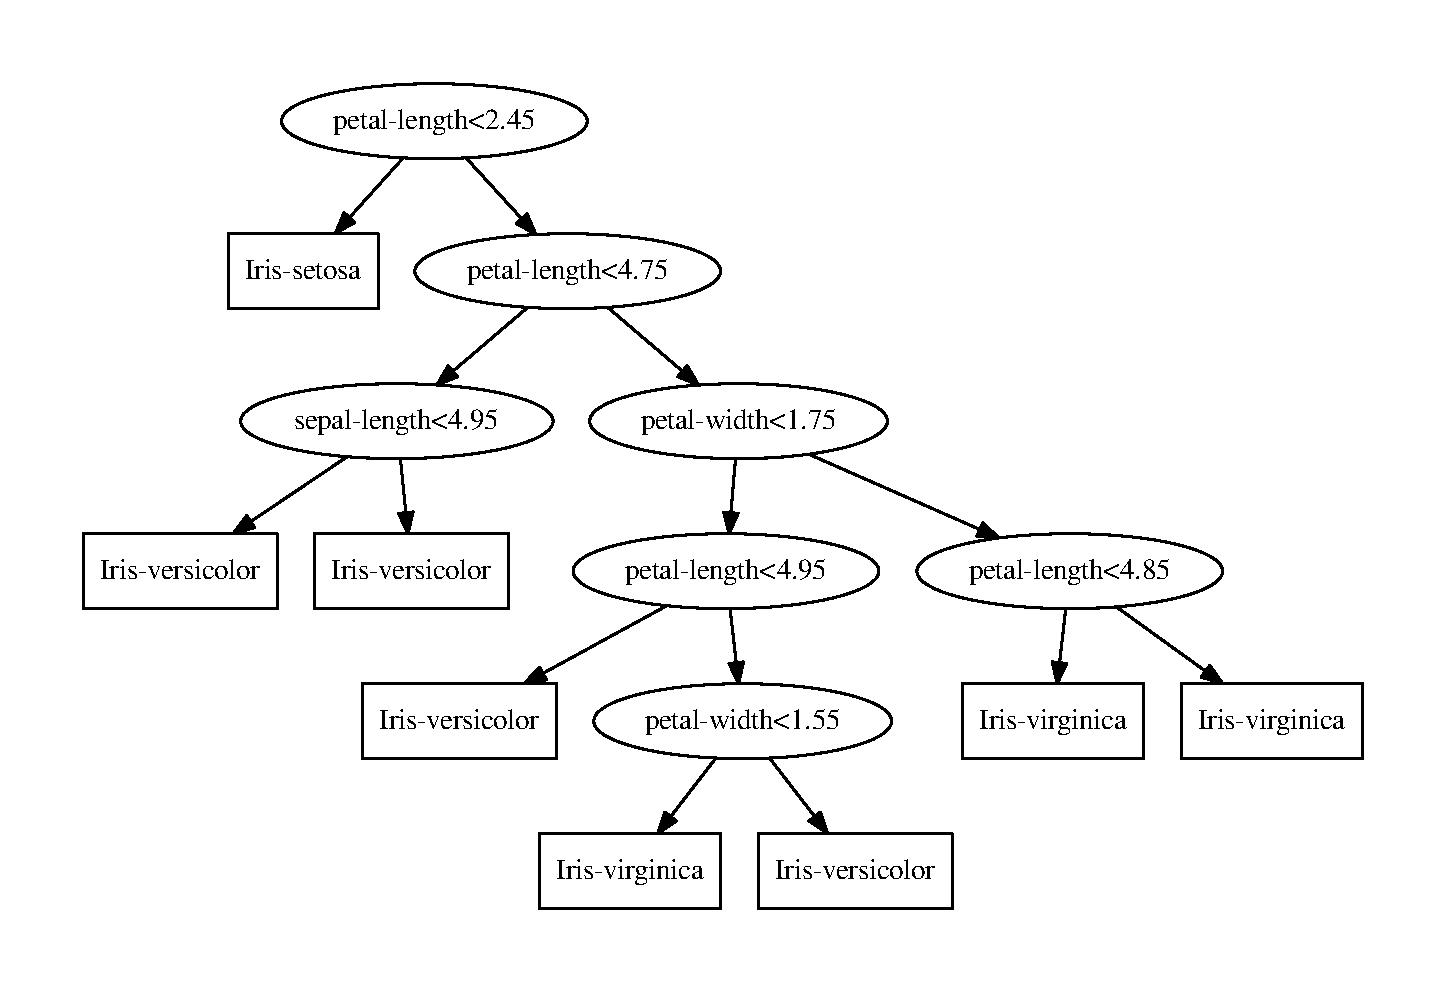
\includegraphics[width=0.75\textwidth]{iris1.pdf}
\caption{One of the learnt trees of the Iris data set}
\label{fig:iris-tree}
\end{figure*}

The full list of rankings and scores can be found in the \texttt{experiment\_results} folder. We
refer the reader there.

% Your document ends here!
\end{document}